\subsection*{Overview}

In order to interact with the robot aside of speech, a web-based \gls{gui} has been designed.
The interface has been made with HTML5\footnote{\texttt{https://github.com/tue-robotics/tue\_mobile\_ui}} and is hosted on the robot itself.
This allows multiple users on different platforms (\eg\ Android, iOS) to access functionality of the robot.

The interface is implemented in JavaScript with AngularJS and it offers a graphical interface to the Robot API\footnote{\texttt{https://github.com/tue-robotics/robot-api}} which exposes all the functionality of the robot.
Figure~\ref{fig:webgui_architecture} gives an overview of the connections between these components.

\begin{figure}[H]
	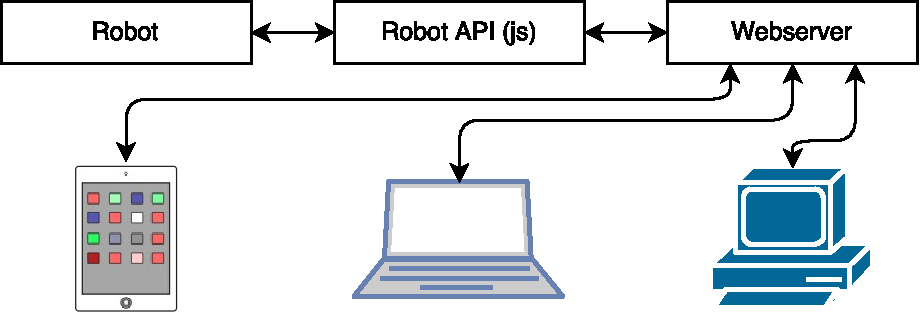
\includegraphics[width=\linewidth]{webgui_architecture}
	\caption{
		Overview of the WebGUI architecture.
		The robot's functionalities are exposed with the Robot API that is implemented in JavaScript.
		The webserver that is hosting the \gls{gui} connects this Robot API to a graphical user interface that is offered to multiple clients on different platforms.}
	\label{fig:webgui_architecture}
\end{figure}

Figure~\ref{fig:gui_actions} gives an example of various user interactions that are possible with the \gls{gui} and the different commands that can be given to the robot while interacting with the virtual scene.

\begin{figure}[H]
	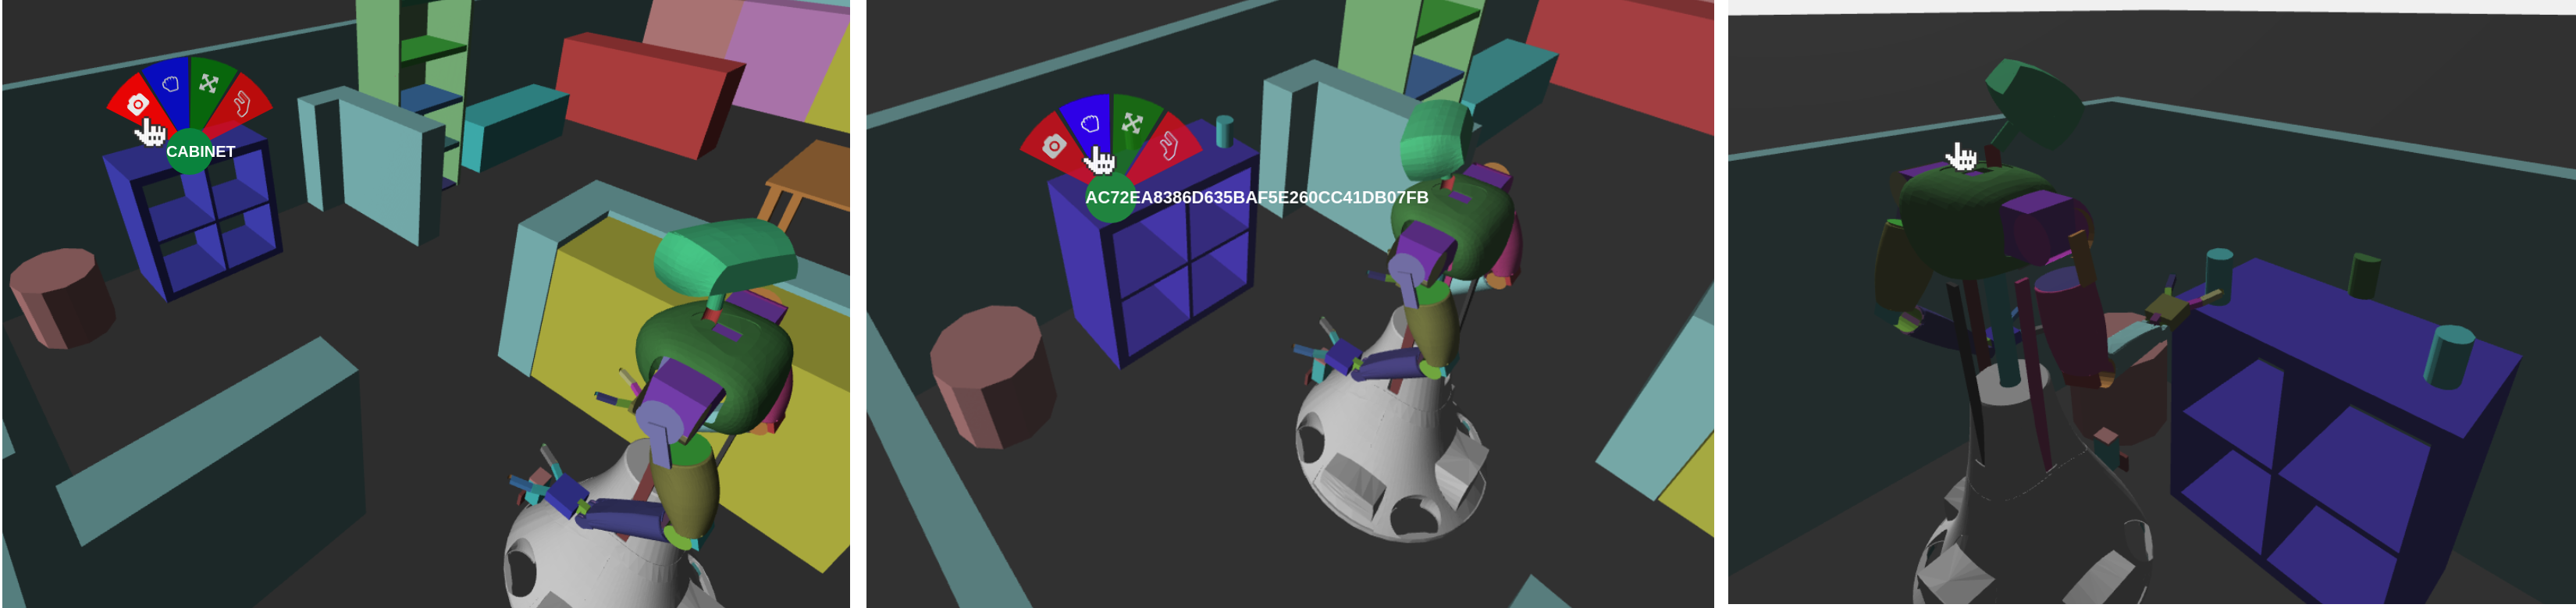
\includegraphics[width=\linewidth]{Figures/gui_actions}
	\caption{
		Illustration of the 3D scene of the WebGUI.
		Users can interact with use of the menu that appears when long pressing an object in the scene.
		On the left figure, the user commands the robot to inspect the selected object, which is the 'cabinet'.
		When the robot has inspected the 'cabinet', it has found entities on top of it.
		In the middle figure a grasp command is given to the robot to pick up an object from the cabinet.
		The last figure show the robot executing that action.}
	\label{fig:gui_actions}
\end{figure}

These actions are passed via the Robot API to the action server that schedules the actions the robot has to perform.
The action server enables various clients to give task commands to the robot without interfering with each other.
Other clients that make use of this action server are Speech and the Natural Language Console, explained in Section~\ref{sec:nli}.
